\documentclass{article}
\usepackage{multicol}
\usepackage[utf8]{inputenc}
\usepackage[T1]{fontenc}      
\usepackage[francais]{babel}
\usepackage{graphicx}
\usepackage{circuitikz}
\usepackage[squaren, Gray]{SIunits}
\usepackage{sistyle}
\usepackage[autolanguage]{numprint}
\usepackage{pgfplots}
\usepackage{geometry}
\usepackage{hyperref}
\usepackage{caption}
\usepackage{amsmath,amssymb,array}
\usepackage{url}
\usepackage{fancyhdr}
\usepackage{layout}
\usepackage[version=3]{mhchem}
\usepackage{array} 
\usepackage{tikz}
	\usetikzlibrary{arrows,shapes,positioning}


\newcommand{\reporttitle}{Analyse dynamique}     % Titre
\newcommand{\reportauthor}{Geoffroy \bsc{Jacquet} \\ Corentin \bsc{Joachim}\\ Léa \bsc{Paulus}} % Auteur
\newcommand{\reportsubject}{Rapport de projet en construction mécanique 1} % Sujet
\newcommand{\HRule}{\rule{\linewidth}{0.5mm}}
\newcommand{\copyrigh}{{\tiny \textregistered}}
\setlength{\parskip}{1ex} % Espace entre les paragraphes

\hypersetup{
    pdftitle={\reporttitle},%
     pdfauthor={\reportauthor},%
    pdfsubject={\reportsubject},%
    pdfkeywords={rapport} {vos} {mots} {clés}
}


\setlength{\headheight}{12pt}
\setlength{\headsep}{12pt}

\pagestyle{fancy}
\lhead{\leftmark{}}
\rhead{LMECA1210 - 2015 - gr11}
\cfoot{\thepage{}}
\begin{document}
\begin{titlepage}

\begin{center}

% Upper part of the page

\textsc{\Large Université Catholique de Louvain}\\[0.5cm]

\textsc{\LARGE Rapport de projet en construction mécanique 1}\\[0.2cm]
\textsc{\LARGE LMECA1210}\\[0.2cm]

% Title
\HRule \\[0.2cm]
{\huge \bfseries Analyse dynamique}\\
\HRule \\[0.2cm]

% Author and supervisor
\begin{center}
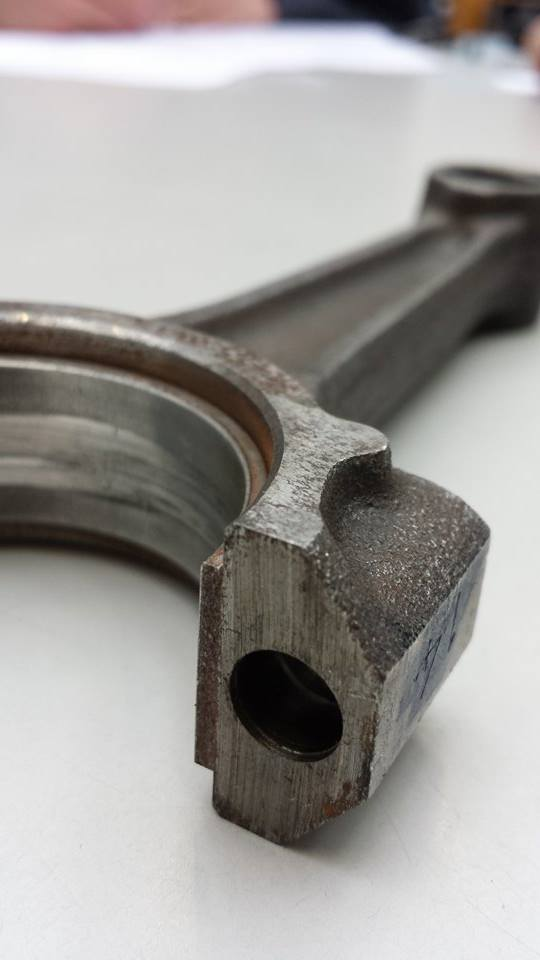
\includegraphics[trim=0cm 8cm 0cm 5cm, clip, width= 15 cm, height= 9.5 cm ]{Schema/bielle2.jpg}
\end{center}
\HRule \\[0 cm]


\begin{minipage}{0.4\textwidth}
\begin{flushleft} \large

\begin{tabular}{l l}

\emph{Auteurs:} & \\
 
Geoffroy & \bsc{Jacquet}\\ 
Corentin & \bsc{Joachim}\\ 
Léa & \bsc{Paulus}

\end{tabular}
\end{flushleft}
\end{minipage}
\begin{minipage}{0.4\textwidth}
\begin{flushright} \large
\emph{Cours:} \\
LMECA1210\\
\emph{Groupe:} \\
11\\
\emph{Professeur:} \\
Hervé \textsc{Jeanmart}
\end{flushright}
\end{minipage}
\vspace{0.3cm}
% Bottom of the page

\begin{minipage}{0.3\textwidth}
\begin{flushleft}

\includegraphics[height=2cm]{Schema/logo_UCL_NEW_janv2013.JPG}
\end{flushleft}
\end{minipage}
\begin{minipage}{0.3\textwidth}
\begin{center}
{\large FSA12BA}\\
{\large \today}
\end{center}
\end{minipage}
\begin{minipage}{0.3\textwidth}
\begin{flushright}

\includegraphics[height=1cm]{Schema/epl-logo.jpg}
\end{flushright}
\end{minipage}
\end{center}
\end{titlepage}
\tableofcontents



\section{Détermination des grandeurs géométriques du moteur}

\begin{center}
\begin{tabular}{|c|c|c|c|}
\hline 
\textbf{Grandeur} & \textbf{Symbole} & \textbf{Valeur} & \textbf{Unités} \\ 
\hline 
Diamètre piston & $D$ & 0.075 & \meter \\ 
\hline 
Longueur manivelle & $R$ & 0.03675 & \meter \\ 
\hline 
Longueur bielle & $L$ & 0.12885 & \meter \\ 
\hline 
Cylindrée & $V_c$ & 324.25 & \cubic\centi\metre \\ 
\hline 
Taux de compression & $\tau$ & 10 & / \\ 
\hline 
\end{tabular} 
\end{center}

Le taux de compression d'un moteur essence à explosion se situe généralement entre 8 et 13, étant généralement assez proche de 10.



\section{Évolution de le pression dans le cylindre}

\begin{center}
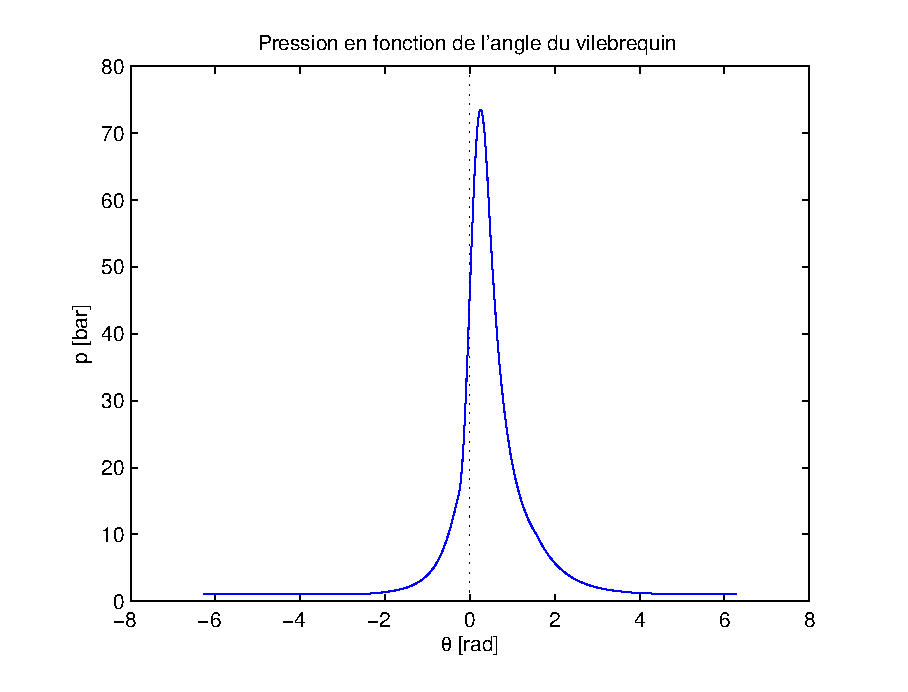
\includegraphics[scale=1]{Schema/pression.eps}
\end{center}



\section{Efforts sur la bielle en fonction de l'angle du vilebrequin}

\subsection{Vitesse : 3000 rpm}
\begin{center}
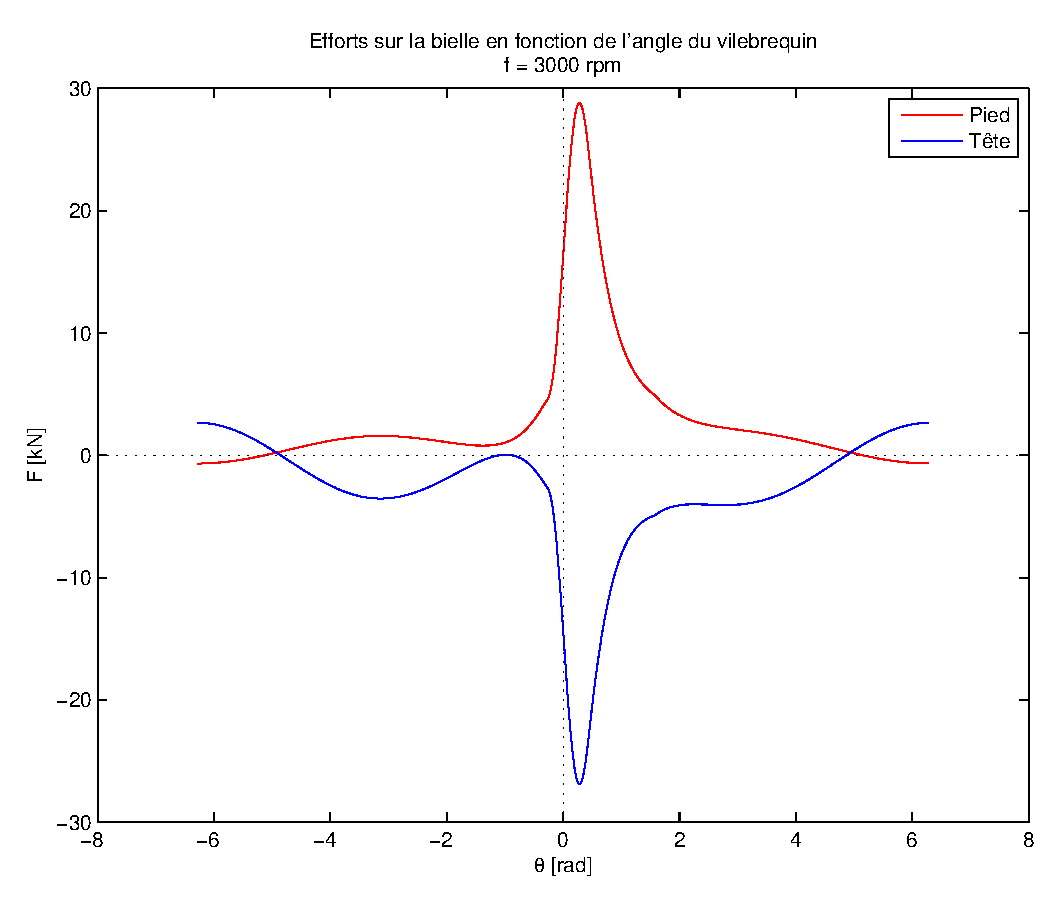
\includegraphics[scale=1]{Schema/forces_3000rpm.eps}
\end{center}

Les deux courbes représentent ici respectivement les efforts sur le pied et la tête de la bielle. Puisque les deux forces sont représentées positives vers le bas, il s'agit de compression lorsque la force sur le pied est positive, et celle sur la tête négative, et de traction dans l'autre cas. 

Les efforts maximums de traction et de compressions sont :

\begin{center}
\begin{tabular}{|c|c|c|}
\hline 
  & \textbf{Pied} & \textbf{Tête} \\ 
\hline 
\textbf{Compression} & \unit{31.397}{ \kilo\newton} & \unit{29.487}{\kilo\newton} \\ 
\hline 
\textbf{Traction} & \unit{0.677}{ \kilo\newton} & \unit{2.65}{ \kilo\newton} \\ 
\hline 
\end{tabular} 
\end{center}

Afin de représenter l'effort total que subit la bielle, il faut donc faire la différence de l'effort sur le pied avec celui sur la tête.

\begin{center}
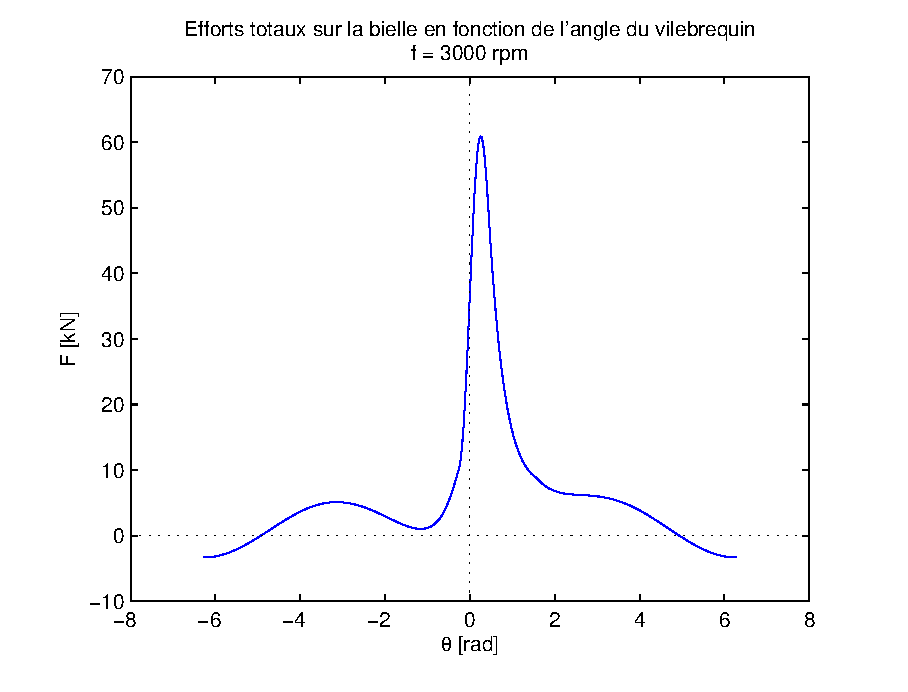
\includegraphics[scale=1]{Schema/forces_tot_3000rpm.eps}
\end{center}

La partie positive du graphe représente un effort de compression tandis que le négative représente de la traction.
Les efforts maximums sont : 

\begin{center}
\begin{tabular}{|c|c|}
\hline 
\textbf{Compression} & \unit{60.884}{ \kilo\newton} \\ 
\hline 
\textbf{Traction} & \unit{3.387}{\kilo\newton} \\ 
\hline 
\end{tabular} 
\end{center}

\subsection{Vitesse : 5000 rpm}

\begin{center}
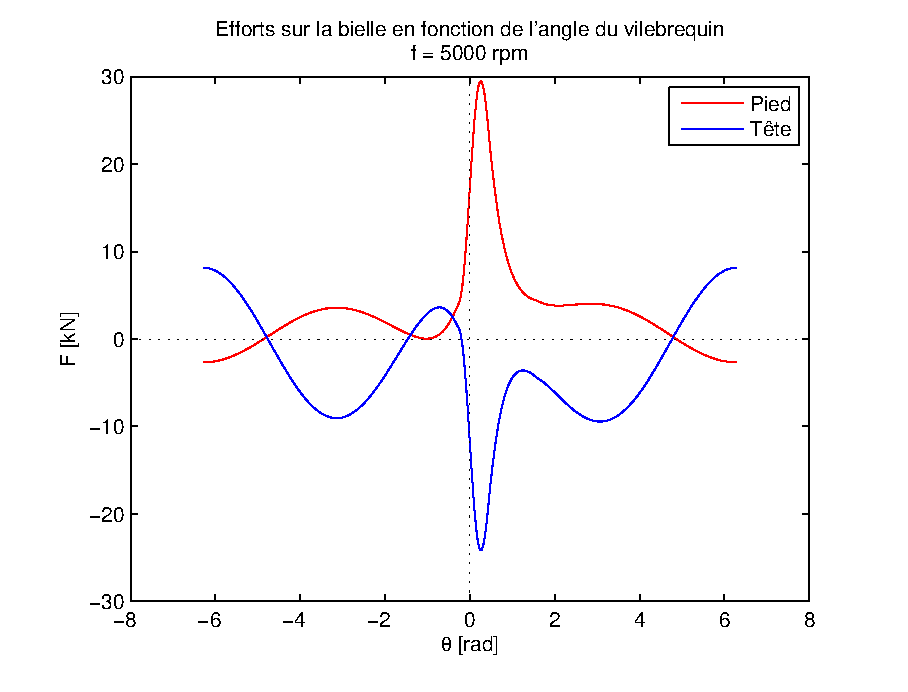
\includegraphics[scale=1]{Schema/forces_5000rpm.eps}
\end{center}

Les conventions sont les mêmes que pour ceux à \unit{3000}{rpm}. Les différents efforts sont : 

\begin{center}
\begin{tabular}{|c|c|c|}
\hline 
  & \textbf{Pied} & \textbf{Tête} \\ 
\hline 
\textbf{Compression} & \unit{29.462}{ \kilo\newton} & \unit{24.162}{ \kilo\newton}\\ 
\hline 
\textbf{Traction} & \unit{2.676}{ \kilo\newton} & \unit{8.157}{\kilo\newton} \\ 
\hline 
\end{tabular} 
\end{center}

A nouveau, l'effort total est représenté.

\begin{center}
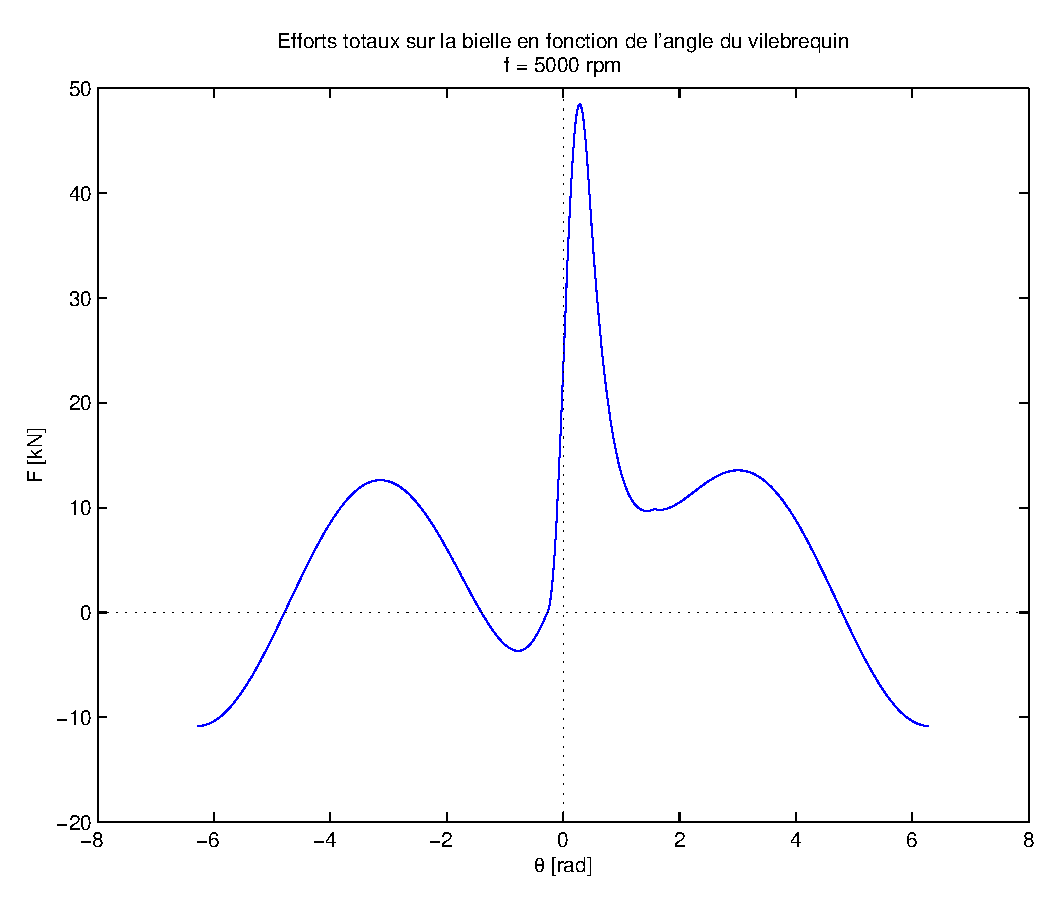
\includegraphics[scale=1]{Schema/forces_tot_5000rpm.eps}
\end{center}

Les efforts maximums sont : 

\begin{center}
\begin{tabular}{|c|c|}
\hline 
\textbf{Compression} & \unit{53.623}{\kilo\newton} \\ 
\hline 
\textbf{Traction} & \unit{10.832}{\kilo\newton} \\ 
\hline 
\end{tabular} 
\end{center}



\section{Justification de la forme en "I"}
La bielle étant contrainte à des efforts de traction et principalement de compression, pour un fonctionnement optimal dans un moteur à haute vitesse il faut que celle-ci soit à la fois élancée, légère tout en étant capable de résister aux sollicitations. La forme qui répond le mieux à l'ensemble de ces critères s'avère être la forme en I.



\section{Dimensionnement de la section de la bielle}

\end{document}